% Apresentação de resultados — Mês 3 (setembro/2026), identidade visual H.IAAC
% Tabelas e figuras: fl-robustness-lab/experiments/make_slides_assets.py (rodar de novo e recompilar)
\documentclass[aspectratio=169,11pt,xcolor=table]{beamer}
\usepackage[utf8]{inputenc}
\usepackage[T1]{fontenc}
\usepackage[brazil]{babel}
\usepackage{booktabs}
\usepackage{graphicx}
\usepackage{amsmath,amssymb}
\usepackage{pifont}
\usetheme{hiaac}
\usetikzlibrary{arrows.meta,positioning}

\newcommand{\ok}{\textcolor{hiaacnavy}{\ding{51}}}
\newcommand{\hl}[1]{\textcolor{hiaacbar}{\textbf{#1}}}

\title{Agente para Detecção de Ataques em Aprendizado Federado}
\subtitle{O que foi feito até aqui e o que os experimentos mostram sobre o RAGNAR}
\author{Marcos Gilliard Oliveira Morais}
\advisor{Leandro A. Villas}
\institute{H.IAAC --- Meta 3 · Setembro de 2026}

\begin{document}

\hiaactitlepage

% =====================================================================
\hiaacsection{Contexto}{O problema e o plano de 12 meses}

\begin{frame}{O problema}
  \begin{columns}[T]
    \column{0.55\textwidth}
    \begin{itemize}
      \item No Aprendizado Federado (FL) o servidor \textbf{não vê os dados}, só as atualizações dos clientes.
      \item Clientes maliciosos podem:
      \begin{itemize}
        \item \textbf{degradar} o modelo (ruído, IPM, LIE, MinMax\dots)
        \item \textbf{inserir comportamento oculto} (backdoor)
        \item \textbf{envenenar os dados} (label flip)
      \end{itemize}
      \item Detectar exige inferir intenção a partir do que é observável.
    \end{itemize}
    \column{0.4\textwidth}
    \begin{block}{Objetivo do projeto}
      Um \textbf{agente de detecção} que combine múltiplos sinais (atualizações e histórico dos clientes) e \textbf{fundamente suas decisões}.
    \end{block}
    \vspace{0.3em}
    \begin{block}{Caso base}
      \textbf{RAGNAR} (Morais et al., 2024): filtro leve com features geométricas + XGBoost.
    \end{block}
  \end{columns}
\end{frame}

\begin{frame}{Plano de 12 meses: onde estamos}
  \centering\footnotesize
  \resizebox{0.95\textwidth}{!}{%
  \begin{tabular}{clll}
    \toprule
    Mês & Atividade & Entregável & Situação \\
    \midrule
    1 (jul) & Revisão de ataques e defesas & Revisão e taxonomia & \ok{} concluído \\
    2 (ago) & Ambiente e cenário de avaliação & Ambiente validado + cenário & \ok{} concluído \\
    \rowcolor{hiaaclight} \textbf{3 (set)} & \textbf{Sinais observáveis} & \textbf{Especificação dos sinais e da lógica} & \textbf{\textcolor{hiaacbar}{em andamento}} \\
    4 (out) & Ataques controlados & Ataques injetáveis & \ok{} adiantado \\
    5 (nov) & Agente (versão inicial) & Protótipo funcional & --- \\
    6 (dez) & Integração à agregação & Pipeline + relatório parcial & --- \\
    7--10 & Detecção, falsos positivos, robustez & Relatórios de avaliação & --- \\
    11--12 & Artigo e relatório final & Manuscrito + repositório & --- \\
    \bottomrule
  \end{tabular}}
\end{frame}

% =====================================================================
\hiaacsection{O que foi feito}{Revisão, ambiente experimental e auditoria}

\begin{frame}{Meses 1 e 2: revisão e ambiente}
  \begin{columns}[T]
    \column{0.45\textwidth}
    \textbf{Revisão sistemática (M1)}
    \begin{itemize}
      \item 16 artigos: BOBA, Blades, FedSecurity, FLGuard, Multi-metrics, XI-DDaBA, RAGNAR\dots
      \item Taxonomia por objetivo, canal (dados/modelo) e furtividade (camadas críticas).
    \end{itemize}
    \column{0.5\textwidth}
    \textbf{\texttt{fl-robustness-lab} (M2)}
    \begin{itemize}
      \item FL simulado em PyTorch: CIFAR-10, 20 clientes, não-IID (Dirichlet).
      \item \textbf{9 ataques}: ruído, sign flip, IPM, LIE, MinMax, MinSum, label flip, backdoor pixel e PGD.
      \item \textbf{9 defesas}: FedAvg, Mediana, Trimmed Mean, (Multi-)Krum, FoolsGold, Multi-métrica, BOBA, RAGNAR.
      \item Métricas: acurácia (MA), sucesso do backdoor (BA), precisão e recall de detecção.
    \end{itemize}
  \end{columns}
\end{frame}

\begin{frame}{Auditoria do ambiente antes de medir}
  \framesubtitle{5 problemas encontrados e corrigidos, todos com testes unitários}
  \footnotesize
  \begin{tabular}{p{4.6cm}p{4.2cm}p{4.2cm}}
    \toprule
    Problema & Impacto & Correção \\
    \midrule
    \texttt{backdoor\_pgd} escalava e voltava à própria norma & idêntico ao backdoor simples & PGD real: treino projetado + escala \\
    BOBA: vértices eram gradientes (sinal/escala opostos) & descartava clientes honestos & deltas de referência por classe \\
    RAGNAR treinado com o ataque avaliado & resultado otimista & treino sem a família avaliada \\
    Parâmetros eram \emph{views} do vetor global & em CPU o treino sobrescrevia o global & cópia explícita \\
    Braço ``ataque visto'' sorteava o treino & o ataque podia nunca ser visto & treino só com o ataque \\
    \bottomrule
  \end{tabular}
\end{frame}

% =====================================================================
\hiaacsection{O RAGNAR funciona?}{Avaliação contra 8 ataques}

\begin{frame}{RAGNAR original: como funciona}
  \centering
  \begin{tikzpicture}[node distance=0.55cm, every node/.style={font=\small},
      box/.style={draw=hiaacnavy, fill=hiaaclight, align=center, minimum height=1.15cm, text width=2.6cm},
      arr/.style={-{Stealth}, hiaacbar, very thick}]
    \node[box] (d) {Pesos enviados pelo cliente};
    \node[box, right=of d] (f) {\textbf{60 features}\\ \scriptsize L1, L2, L3 dos pesos e sua variação, \textbf{por camada}};
    \node[box, right=of f] (c) {MinMax + XGBoost\\ \scriptsize exclui se $P > 0{,}9$};
    \node[box, right=of c] (a) {Agrega os demais\\ \scriptsize (a partir do round 2)};
    \draw[arr] (d) -- (f); \draw[arr] (f) -- (c); \draw[arr] (c) -- (a);
    \node[box, below=0.8cm of c, text width=5cm] (b) {\textbf{Treino offline}: simulações prévias completas (muitas épocas e rounds); depois \textbf{congelado}};
    \draw[arr, dashed] (b) -- (c);
  \end{tikzpicture}
  \vspace{0.6em}
  \begin{itemize}
    \item Pergunta-chave: um classificador \textbf{supervisionado} reconhece ataques que \textbf{não viu} no treino?
  \end{itemize}
\end{frame}

\begin{frame}{Reimplementação v1 do laboratório vs. original}
  \framesubtitle{A primeira rodada avaliou uma versão diferente do método}
  \centering\small
  \begin{tabular}{lll}
    \toprule
     & RAGNAR original & Reimplementação v1 \\
    \midrule
    Features & 60, por camada (pesos) & 4, no vetor inteiro (delta vs. média) \\
    Normalização & MinMax & nenhuma \\
    Limiar & 0,9 & 0,5 \\
    Treino & simulações completas & 5 rounds a partir do modelo inicial \\
    Início & round 2 & round 1 \\
    \bottomrule
  \end{tabular}\\[0.8em]
  \raggedright\footnotesize Os resultados a seguir valem para a \textbf{v1}; a versão fiel já está implementada no laboratório (\texttt{ragnar\_original}).
\end{frame}

\begin{frame}{Experimento 1: v1 contra todos os ataques}
  \begin{itemize}
    \item 8 ataques, semente 42: 20 clientes, 20\% maliciosos (10\% nos backdoors), $\alpha=0{,}5$, 40 rounds.
  \end{itemize}
  \vspace{0.3em}
  \centering
  \begin{tabular}{ll}
    \toprule
    Braço & Pergunta \\
    \midrule
    FedAvg (sem defesa) & Quanto estrago o ataque faz? \\
    RAGNAR v1, ataque \textbf{não visto} ($nv$) & Generaliza para um ataque novo? \\
    Sem ataque & Teto de acurácia \\
    \bottomrule
  \end{tabular}
  \vspace{0.6em}
  \begin{block}{Por que ``não visto'' importa}
    Na prática ninguém sabe de antemão qual ataque vai sofrer.
  \end{block}
\end{frame}

\begin{frame}{Resultados: RAGNAR v1 vs. sem defesa}
  \centering
  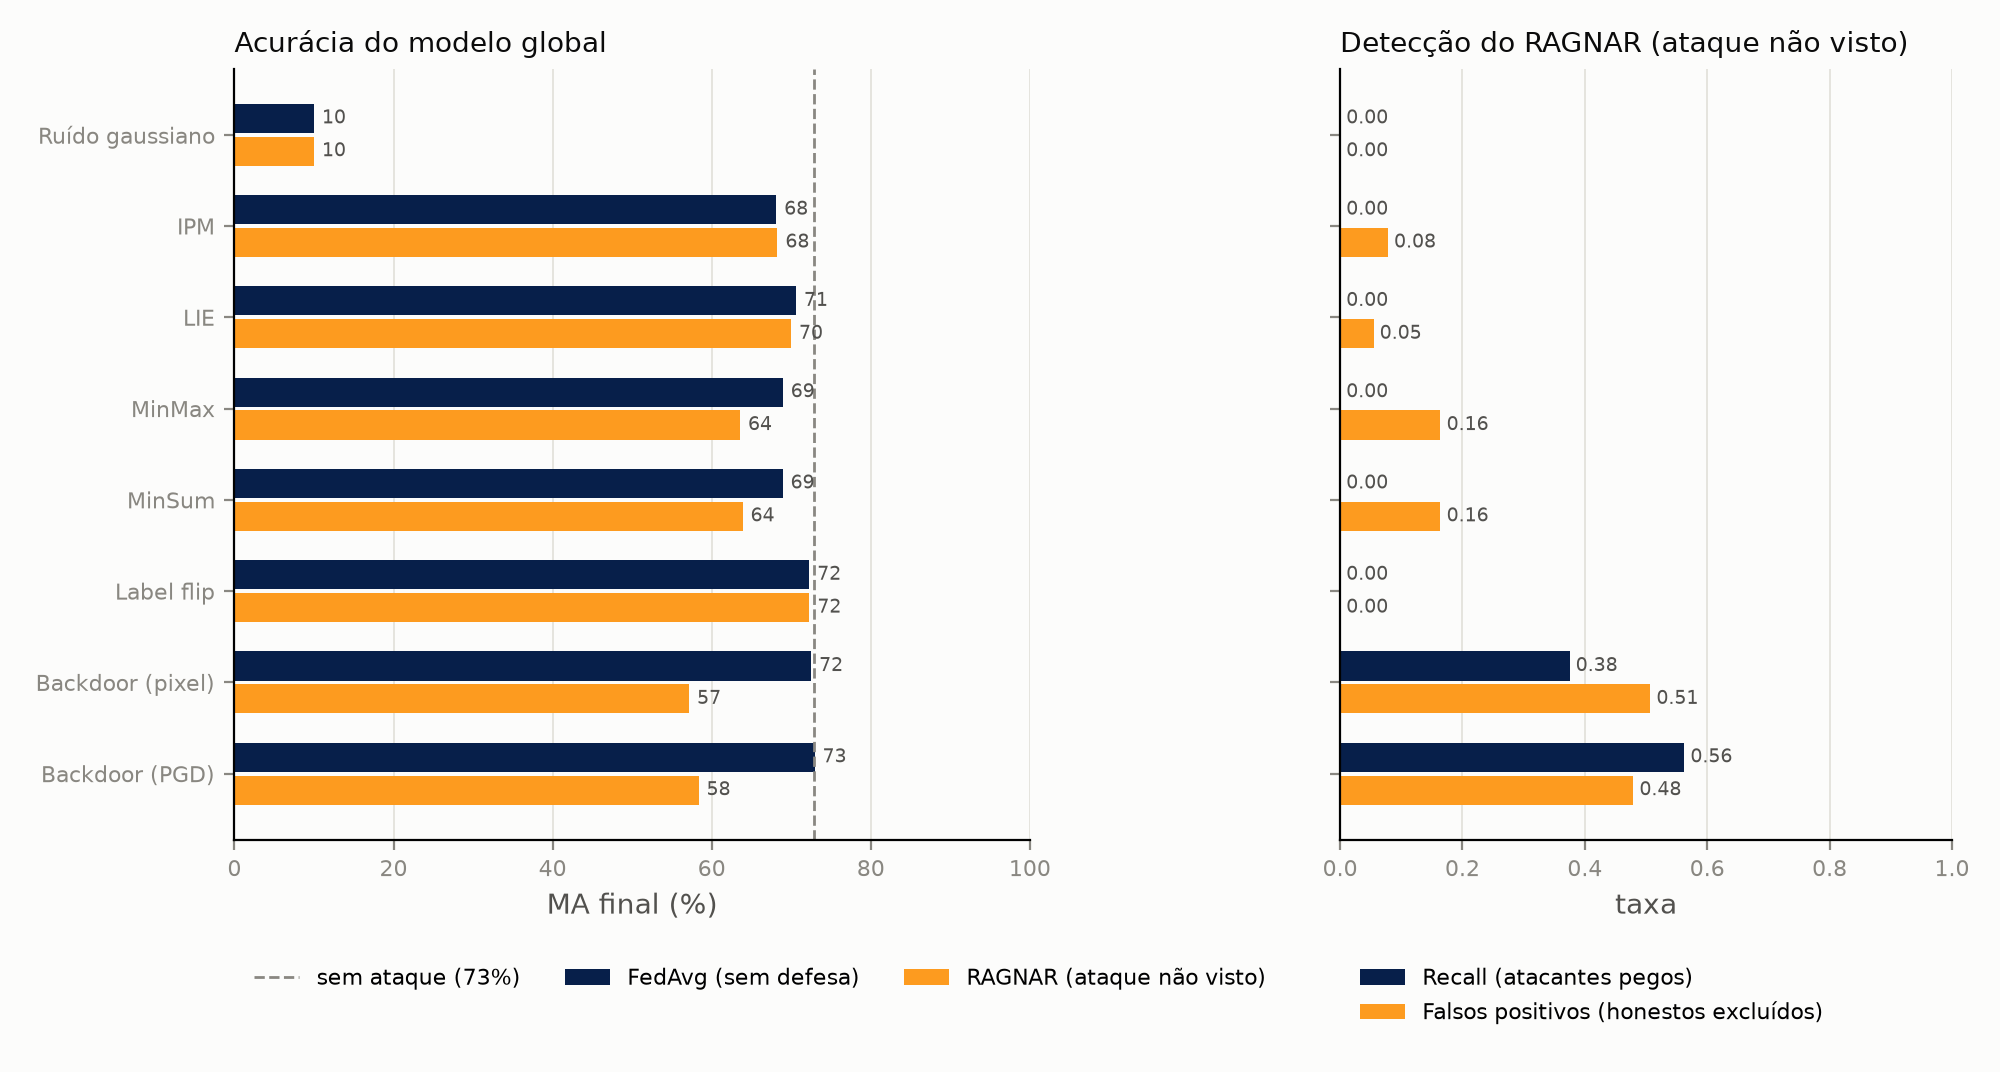
\includegraphics[width=0.95\textwidth,height=0.74\textheight,keepaspectratio]{figuras/ragnar_vs_fedavg.png}
\end{frame}

\begin{frame}{Resultados em números}
  \centering\small
  \resizebox{0.92\textwidth}{!}{\begin{tabular}{lrrrrrr}
\toprule
Ataque & MA FedAvg & MA RAGNAR$_{nv}$ & BA FedAvg & BA RAGNAR$_{nv}$ & Recall$_{nv}$ & FP$_{nv}$ \\
\midrule
Ruído gaussiano & 10.0 & 10.0 & -- & -- & 0.00 & 0.00 \\
IPM & 68.1 & 68.3 & -- & -- & 0.00 & 0.08 \\
LIE & 70.6 & 70.0 & -- & -- & 0.00 & 0.05 \\
MinMax & 68.9 & 63.6 & -- & -- & 0.00 & 0.16 \\
MinSum & 68.9 & 63.9 & -- & -- & 0.00 & 0.16 \\
Label flip & 72.3 & 72.3 & -- & -- & 0.00 & 0.00 \\
Backdoor (pixel) & 72.5 & 57.2 & 75.4 & 93.8 & 0.38 & 0.51 \\
Backdoor (PGD) & 72.9 & 58.4 & 66.3 & 80.5 & 0.56 & 0.48 \\
\midrule
\multicolumn{7}{l}{\footnotesize Sem ataque (FedAvg): MA = 72.8\%} \\
\bottomrule
\end{tabular}
}\\[0.6em]
  \footnotesize MA = acurácia (\%) · BA = sucesso do backdoor (\%, menor é melhor) · FP = fração de honestos excluídos · uma semente
\end{frame}

\begin{frame}{O que o Experimento 1 mostra}
  \begin{alertblock}{RAGNAR v1, ataque não visto: não protege, e às vezes piora}
    \begin{itemize}
      \item \textbf{Backdoors}: exclui $\sim$50\% dos \textbf{honestos} $\Rightarrow$ MA 72\%$\to$57\% e o backdoor fica \textbf{mais} forte (BA 75\%$\to$94\%).
      \item \textbf{Ataques de modelo} (IPM, LIE, MinMax, MinSum): recall 0.
      \item \textbf{Label flip}: nenhuma detecção.
      \item \textbf{Ruído gaussiano}: todos colapsam para 10\%, inclusive com o RAGNAR.
    \end{itemize}
  \end{alertblock}
  \vspace{0.4em}
  Próxima pergunta: \textbf{por quê?} Falta informação nas features, ou o classificador aprende a regra errada?
\end{frame}

\begin{frame}{Modelo pré-treinado do RAGNAR original}
  \framesubtitle{Teste de compatibilidade: mesma CNN e mesmo otimizador (Adam, lr=$10^{-3}$)}
  \begin{columns}[T]
    \column{0.5\textwidth}
    \begin{itemize}
      \item Carregamos \texttt{CLASSIFICADOR\_XGB\_CNN} + \texttt{MINMAX\_XGB\_CNN} do ataca\_FEDML.
      \item \textbf{68--95\%} das features caem fora da faixa do MinMax, mesmo em \textbf{clientes honestos}.
      \item Ex.: L1 de \texttt{fc2.w} em $-24$ e variações por round de 3 a 12 (faixa válida: 0 a 1).
      \item Não detectou nem o ruído gaussiano: $P_{\max}=0{,}84 < 0{,}9$.
    \end{itemize}
    \column{0.45\textwidth}
    \begin{alertblock}{Leitura}
      Features \textbf{absolutas} (normas dos pesos) prendem o classificador ao ambiente em que foi treinado: dados, normalização, nº de clientes, passos locais.\\[0.4em]
      Não é possível avaliá-lo fora do ataca\_FEDML.
    \end{alertblock}
  \end{columns}
\end{frame}

% =====================================================================
\hiaacsection{Por que falha?}{Análise de discriminabilidade dos sinais}

\begin{frame}{Experimento 2: quanto cada sinal separa?}
  \begin{columns}[T]
    \column{0.52\textwidth}
    19 sinais por cliente e por round, em 6 famílias:
    \begin{itemize}\small
      \item geometria do RAGNAR v1 (L1, L2, L3, cosseno)
      \item geometria robusta (mediana, Mahalanobis, Krum)
      \item conluio (similaridade entre clientes)
      \item camada crítica (\texttt{fc1})
      \item referência no servidor (holdout, FLTrust)
      \item histórico entre rounds
    \end{itemize}
    \column{0.42\textwidth}
    \begin{block}{Protocolo}
      \small
      \begin{itemize}
        \item \textbf{Agregação oráculo}: mede detectabilidade, não estrago.
        \item \textbf{AUC dentro de cada round}, média entre rounds.
        \item 0,5 = não separa · 1,0 = separa perfeitamente.
      \end{itemize}
    \end{block}
  \end{columns}
\end{frame}

\begin{frame}{Mapa de discriminabilidade}
  \centering
  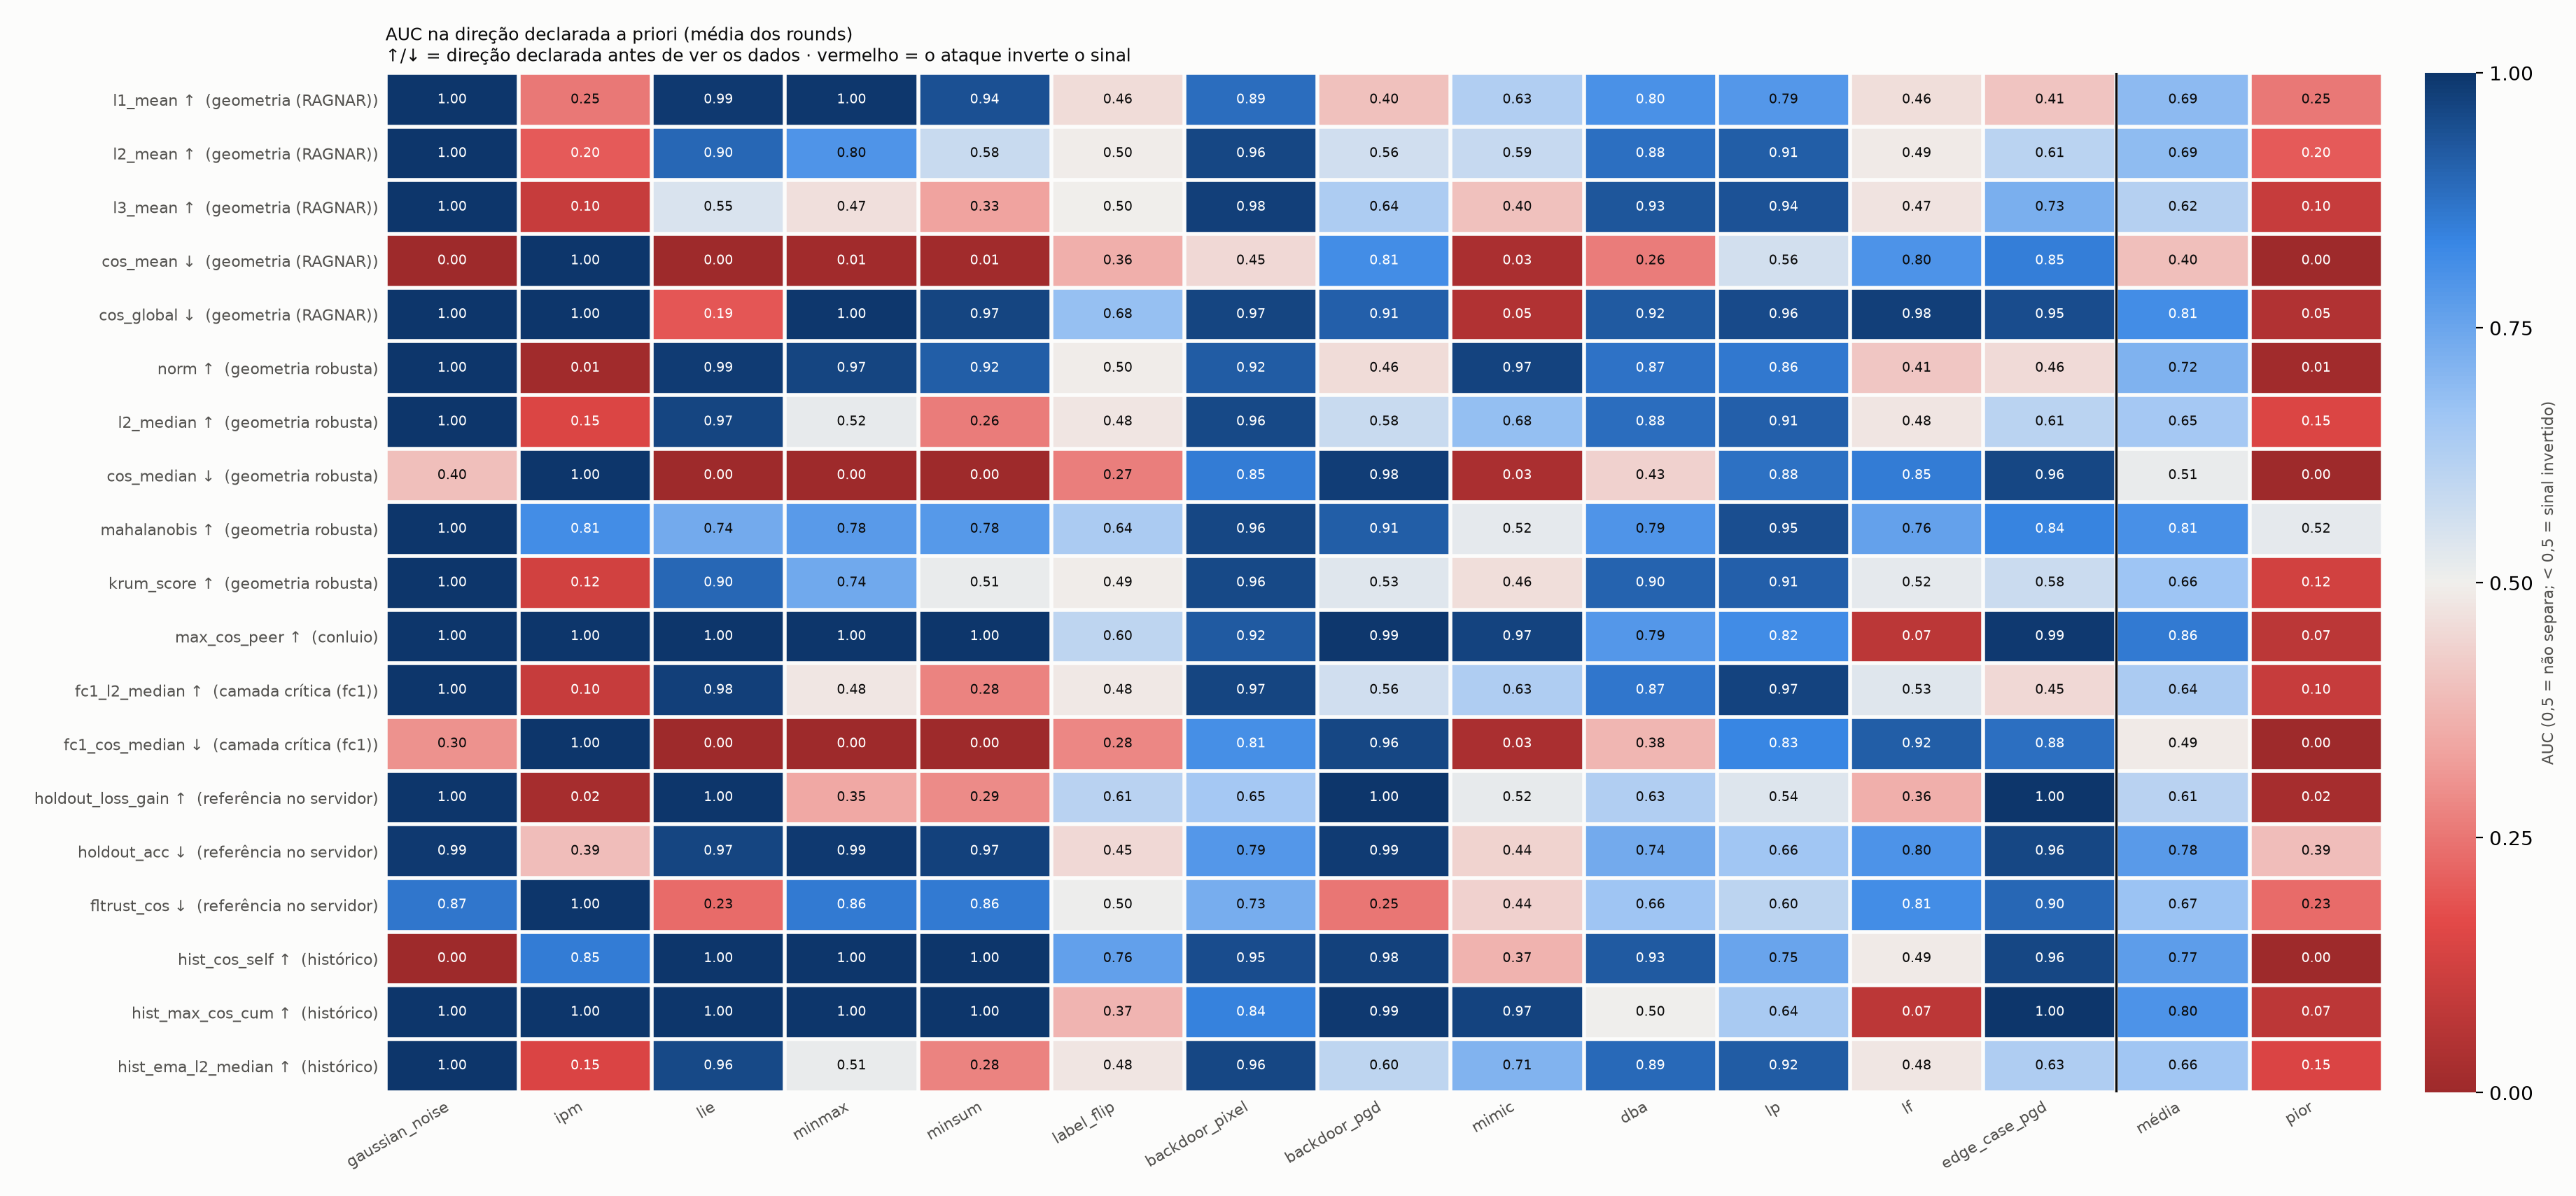
\includegraphics[height=0.78\textheight,keepaspectratio]{figuras/heatmap_signals.png}
\end{frame}

\begin{frame}{Achados da análise de sinais}
  \begin{enumerate}
    \item \textbf{Ataques de modelo são fáceis de separar}: vários sinais com AUC $\approx$ 1,0, inclusive os do RAGNAR v1.\\
      {\footnotesize (parte vem de os atacantes enviarem vetores idênticos --- atacante adaptativo no mês 10)}
    \item \textbf{Normas falham contra o backdoor PGD} (0,56--0,64): o ataque limita a norma. O que pega: efeito no holdout (1,00), consistência entre rounds (0,98), cosseno com a mediana (0,98).
    \item \textbf{Label flip é o mais difícil}: nenhum sinal passa de 0,76; o melhor é de \textbf{histórico}.
  \end{enumerate}
  \vspace{0.3em}
  \begin{block}{Consequência}
    Nos ataques de modelo a informação \textbf{existe} nas features: a falha é do \textbf{classificador}.
  \end{block}
\end{frame}

\begin{frame}{A regra muda ao longo do treino}
  \begin{columns}[c]
    \column{0.48\textwidth}
    Cosseno com a média (feature da v1), backdoor pixel:\\[0.6em]
    \centering\small
    \begin{tabular}{lcl}
      \toprule
      Fase & AUC & Malicioso tem cosseno \\
      \midrule
      rounds 2--7 & \textbf{0,21} & \emph{menor} \\
      rounds 8--15 & \textbf{0,87} & \emph{maior} \\
      \bottomrule
    \end{tabular}\\[0.4em]
    \raggedright\footnotesize a média (0,55) esconde um sinal forte que \textbf{inverte de sentido}
    \column{0.46\textwidth}
    \begin{alertblock}{Por que isso quebra a v1}
      \begin{itemize}
        \item A v1 treinava só com \textbf{5 rounds} a partir do modelo inicial.
        \item Aprende a regra da fase inicial e a aplica depois, quando ela já se inverteu.
        \item Features \textbf{absolutas}: a escala muda com o treino --- o mesmo problema do modelo pré-treinado.
      \end{itemize}
    \end{alertblock}
  \end{columns}
\end{frame}

\begin{frame}{Experimento 3: treinado cedo, testado tarde}
  \begin{columns}[T]
    \column{0.5\textwidth}
    \centering\small
    \resizebox{\linewidth}{!}{\begin{tabular}{llrrr}
\toprule
Sinais & Normalização & AUC & Recall & Falsos pos. \\
\midrule
RAGNAR-4 & nenhuma & 0.52 & 0.37 & 0.39 \\
 & z robusto & 0.68 & 0.41 & 0.06 \\
 & rank & 0.60 & 0.18 & 0.06 \\
\addlinespace
ampliado-10 & nenhuma & 0.93 & 0.73 & 0.04 \\
 & z robusto & 0.90 & 0.66 & 0.04 \\
 & rank & 0.87 & 0.64 & 0.02 \\
\addlinespace
robusto & nenhuma & 0.76 & 0.36 & 0.20 \\
 & z robusto & 0.86 & 0.24 & 0.03 \\
 & rank & 0.79 & 0.18 & 0.02 \\
\addlinespace
todos & nenhuma & 0.91 & 0.67 & 0.01 \\
 & z robusto & 0.96 & 0.71 & 0.01 \\
 & rank & 0.90 & 0.70 & 0.01 \\
\bottomrule
\end{tabular}
}\\[0.3em]
    \raggedright{\footnotesize Treino: rounds 2--5 · teste: $\geq$ 8 · ataque não visto · limiar 0,5 · média de 8 ataques}
    \column{0.45\textwidth}
    \begin{itemize}
      \item \textbf{Features da v1}, sem normalização: AUC \hl{0,48} (acaso) e \hl{44\%} de honestos excluídos.
      \item \textbf{z-score robusto no round}: AUC 0,68 e 3\% de falsos positivos, com as mesmas 4 features.
      \item \textbf{Sinais adicionais}: AUC 0,91.
      \item Label flip continua sem detecção.
    \end{itemize}
  \end{columns}
\end{frame}

% =====================================================================
\hiaacsection{Formulações robustas}{Sinais que não dependem da escala nem da fase do treino}

\begin{frame}{Conceitos matemáticos mais robustos}
  \footnotesize
  \begin{tabular}{p{4.4cm}p{6.6cm}p{1.8cm}}
    \toprule
    Problema observado & Conceito & Situação \\
    \midrule
    Referência = média (ruptura 0) & \textbf{Mediana geométrica} (Weiszfeld), ruptura 50\% & em teste \\
    Escala muda com o treino/ambiente & \textbf{z-score robusto} (mediana/MAD) ou rank & \ok{} validado \\
    Mahalanobis contaminado & \textbf{MCD} (Rousseeuw) & em teste \\
    Backdoors em conluio & \textbf{Assinaturas espectrais} (Tran et al., 2018) & em teste \\
    PGD limita a norma & \textbf{Concordância de sinais} (SignGuard/RLR) & em teste \\
    Label flip afeta uma classe & \textbf{Perda por classe} no holdout, divergência JS & em teste \\
    Sinal fraco mas persistente & \textbf{CUSUM} / SPRT entre rounds & em teste \\
    Limiar fixo não controla FP & \textbf{Predição conforme} (FP $\leq \alpha$) & mês 9 \\
    \bottomrule
  \end{tabular}
\end{frame}

% =====================================================================
\hiaacsection{Próximos passos}{Entregável do mês 3 e rumo do agente}

\begin{frame}{Entregável do mês 3 e rumo do agente}
  \begin{columns}[T]
    \column{0.46\textwidth}
    \textbf{Especificação dos sinais (M3)}
    \begin{itemize}
      \item Catálogo de sinais com evidência por ataque.
      \item Formulação atual vs. robusta.
      \item Lógica de decisão do agente.
      \item Comparação justa: RAGNAR original (treino completo) vs. treino curto, no mesmo ambiente.
    \end{itemize}
    \column{0.48\textwidth}
    \textbf{Agente = RAGNAR evoluído (M5--M6)}
    \begin{itemize}
      \item \textbf{Sinais}: + direção robusta, camada crítica, holdout por classe, histórico.
      \item \textbf{Normalização} dentro do round (independe do ambiente).
      \item \textbf{Treino} cobrindo todas as fases do FL.
      \item \textbf{Evidência acumulada} entre rounds (CUSUM).
      \item \textbf{Explicação}: contribuição de cada sinal.
    \end{itemize}
  \end{columns}
\end{frame}

\begin{frame}{Limitações}
  \begin{itemize}
    \item \textbf{Uma semente}: diferenças de 1--2 pontos podem ser ruído.
    \item \textbf{Cenário único}: CIFAR-10, $\alpha=0{,}5$, 20\% de atacantes; falta label skew severo ($\alpha=0{,}1$).
    \item \textbf{Experimento 1 com a v1}, não com o RAGNAR original.
    \item \textbf{Análise de sinais} nos rounds iniciais e com agregação oráculo.
    \item \textbf{Ataques não adaptativos}: vetores idênticos facilitam a detecção por conluio.
    \item \textbf{Sem comparação} com BOBA, Multi-Krum etc.
  \end{itemize}
\end{frame}

\hiaacclosing{{\LARGE\bfseries Obrigado!}\\[0.8em]
  {\small Código, resultados e esta apresentação: \texttt{fl-robustness-lab/}}}

\end{document}
